\section{Data}\label{sec:data}

\paragraph{Corpora and languages} This study uses two public, human-annotated NER corpora with BIO tags (Table~\ref{tab:data}). NCHLT NER~\cite{eiselen2016} covers South African government text and has no official splits, therefore we shuffle each language once with a fixed seed and save one 80/10/10 train/dev/test split. MasakhaNER~2.0~\cite{adelani2022} covers news, and we keep its published splits. The six targets form two clusters: the Nguni languages isiZulu (zul), isiXhosa (xho) and siSwati (ssw), which are written conjunctively, and the Sotho-Tswana languages Sepedi (nso), Sesotho (sot) and Setswana (tsn), which are written disjunctively. Swahili (swa) and Chichewa (nya) are Bantu but not Southern Bantu languages, are written conjunctively, and serve only as sources. This gives nine test sets, six from NCHLT and three from MasakhaNER. isiZulu, isiXhosa and Setswana appear in both corpora, and these are the only cells in which language and corpus are fully crossed.

\begin{table}[t]
\centering\footnotesize
\caption{Corpora. NCHLT sizes are from our seeded 80/10/10 split after deduplication; MasakhaNER sizes are the downloaded splits before deduplication.}
\label{tab:data}
\begin{tabular}{@{}>{\raggedright}p{1.8cm}>{\raggedright}p{1.85cm}>{\raggedright\arraybackslash}p{4.15cm}@{}}
\toprule
Corpus & Languages & Size, labels, licence\\
\midrule
NCHLT NER (government) & zul, xho, ssw, nso, sot, tsn & $\geq$15,000 annotated entity tokens per language; train/dev/test: zul 8,680/1,085/1,086; xho 4,939/617/618; ssw 8,409/1,051/1,052; nso 5,584/698/698; sot 7,486/935/937; tsn 6,214/776/778; PER, LOC, ORG, MISC; CC BY 2.5 ZA\\
\addlinespace
MasakhaNER 2.0 (news) & zul, xho, tsn; swa, nya (sources only) & train/dev/test: zul 5,848/836/1,670; xho 5,718/817/1,633; tsn 3,489/499/996; train swa 6,593, nya 6,250; PER, LOC, ORG, DATE; CC BY-NC 4.0\\
\bottomrule
\end{tabular}
\end{table}

\paragraph{Label harmonisation and source cap} All experiments use the PER, LOC and ORG types. NCHLT \texttt{MISC} and MasakhaNER \texttt{DATE} spans, which make up 4--11\% of NCHLT tokens, are masked, meaning that they are excluded from the loss and from scoring instead of being relabelled as non-entities. Each source is capped at 3,000 training sentences, resampled with each seed. However, the cap equalises sentences and not entities: the estimated number of PER/LOC/ORG spans per 3,000 sentences ranges from about 5,600 (Swahili) to 1,900 (NCHLT Setswana), and Section~\ref{sec:res-robust} tests whether this matters.

\paragraph{Deduplication} The first complete run (v1) contained duplicate sentences that leaked between training and test data. We detected them by exact match on lower-cased, whitespace-normalised token sequences and removed 922 NCHLT sentences (0.9--2.6\% per language) and 626 MasakhaNER training and development sentences (at most 8.2\%, for the isiXhosa training data), while the MasakhaNER test sets keep their published sizes. All results come from the deduplicated run (v2). Removing the leakage lowered the most affected in-language scores (MasakhaNER isiXhosa 89.5\ra 88.1; NCHLT Setswana 81.6\ra 78.6), but it did not change the direction of any finding.

\paragraph{Exposure and tokenizer fertility} Following AfroXLMR's adaptation corpus~\cite{alabi2022}, isiZulu, isiXhosa and Sesotho are treated as \emph{seen} targets and siSwati, Sepedi and Setswana as \emph{unseen} targets. Tokenizer fertility, the number of subwords per word on the training data, is 1.51 for Swahili, 1.77--1.87 for the Sotho-Tswana corpora, 2.25 for Chichewa and 2.43--2.78 for the Nguni corpora (Figure~\ref{fig:fertility}). Furthermore, the NCHLT Sesotho corpus is anomalous: its in-language score is 59.5 here and 55.6 in SERENGETI~\cite{adebara2023}, against about 77--81 for Setswana and Sepedi~\cite{adebara2023,hanslo2022}.

\begin{figure}[t]
\centering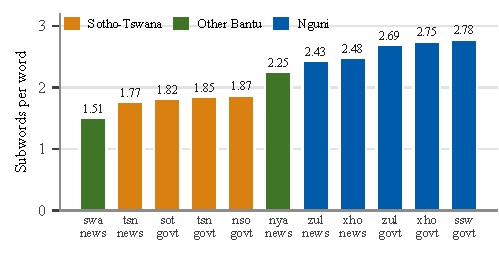
\includegraphics[width=\columnwidth]{figures/fertility_by_corpus}
\caption{AfroXLMR tokenizer fertility (subwords per word) on each training corpus, coloured by language group. Swahili's fertility is closer to that of the Sotho-Tswana corpora than Chichewa's or the Nguni corpora's.}
\label{fig:fertility}
\end{figure}
